\chapter[Introduction]{Introduction}
\label{Chap:Introduction}

\section{Topic Definition}
In recent years, growth of the Internet of Things (IoT) has led to an unprecedented increase in the number of internet-connected devices, with estimates suggesting that there will be over 75 billion IoT devices by 2025 \cite{Alam2018}. However, this growth has brought to attention the importance of network security in embedded systems, especially where sensitive data is handled. Cyber-attacks targeting IoT devices have become more sophisticated and frequent, with the number of IoT attacks increasing by 300\% in 2019 alone \cite{Michael2019}. The financial impact of these attacks is staggering, with the annual cost of data breaches speculated to reach \$10.5 trillion by 2025 \cite{Morgan2020}. 

Trends in the IoT space such as edge computing, 5G networks, and artificial intelligence (AI) are sky-rocketing the demand for highly-performant processing solutions \cite{Nuttall2018} while traditional software-based security approaches often struggle to keep up with the real-time requirements and resource constraints of IoT devices \cite{Frustaci2018}. Frustaci et al. \cite{Frustaci2018} highlight the limited memory, processing power, and energy resources of IoT devices make it challenging to implement strong security measures using software alone without compromising performance and battery life. This is where FPGAs can offer a solution. By leveraging the flexibility of FPGAs, it is possible to create an optomised and dedicated network security solution.

This thesis proposes the development of a RISC-V softcore processor that prioritises network security in embedded IoT applications. The use of RISC-V has several advantages over other contemporary architectures. For one, it is an open-source instruction set architecture that is concise, modular, and extensible \cite{Patterson2017}. Its open nature allows for customization of the processor design to meet specific requirements, while its modular design enables the addition of custom instructions and extensions to emphasise security-related tasks \cite{Waterman2016}. With this, the project aims to show how a dedicated solution can be highly-performant while also mitigating potential threats at the hardware level.

\subsection{Aims}
A successful FPGA-based softcore processor for network security is:
\begin{enumerate}
    \item Secure within networks.
    \item Low-latency.
    \item Power efficient.
    \item Resource-minimising.
    \item And scalable to peripherals/add-ons.
\end{enumerate}

\subsection{Key Performance Indicators}
The previous aims will be evaluated against the following criteria:
\begin{enumerate}
    \item\textbf{Network Security:}\newline Packet sniffing and interception testing will be conducted against the ingoing/outgoing encrypted packets, see section ~\ref{sec:Project Overview}. The subsequent key performance indicators also contribute to overall network security.
    \item\textbf{Processing Latency:}\newline Packet processing time will be measured under idle, average and peak network conditions. This will involve testing the system with differing packet amounts and sizes with security features enabled/disabled to assess any performance bottlenecks. The latency results will also be compared with pre-existing security solutions to benchmark the performance of the softcore processor.
    \item\textbf{Power Efficiency:}\newline Power consumption will be measured also during idle, average, and peak loads. The energy efficiency ratio (performance per watt) will be calculated to provide a standardized metric for comparison. The power efficiency of the system will be compared with other FPGA-based and software-based solutions to assess its relative performance. There's also the possibility of a thermal camera will be used to visualise the heat radiation from the FPGA. There is also the possibility of using the integrated temperature sensor on the Arty S7 Board \cite{ArtyS7RefManual} for plots.
    \item\textbf{Resource Utilisation:}\newline Resource utilization will be evaluated by measuring the counts of FPGA resources in the FPGA design software, such as look-up tables (LUTs), flip-flops and block RAM (BRAM). Memory and CPU utilization on the target IoT devices will also be observed to ensure the system does not overburden the resources available.
\end{enumerate}

\section{Project Overview}
\label{sec:Project Overview}
This section will now pertain to the complete hardware and software stack of of the proposed solution. A high-level overview of which can be seen in figure \ref{Fig:1}.
\begin{figure}[ht]
    \begin{center}
        \caption{High-Level Network Overview}
        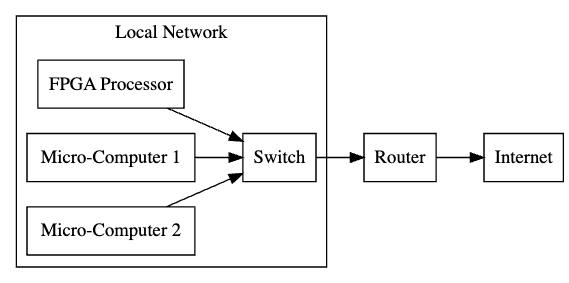
\includegraphics[width=0.8\textwidth]{./Figures/Network_Overview.png}
        \label{Fig:1}
    \end{center}
\end{figure}

Here, the local network refers to the arrangement of the edge devices in the network (left-hand side). It consists of the project's primary focus, the RISC-V softcore processor as well as a Kubernetes cluster network which is scalable to any number of test edge devices. On the right hand side is the router which will interface the local network with the external internet structure, allowing external communications.

\begin{figure}[h]
    \begin{center}
    \caption{High-Level FPGA Architecture Overview}
    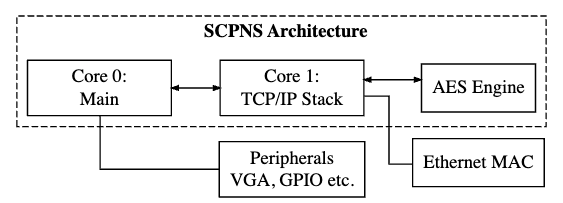
\includegraphics[width=0.8\textwidth]{./Figures/FPGA_Architecture_High_Level.png}
    \label{Fig:2}
    \end{center}
\end{figure}

\subsection{Softcore Processor for Network Security, (SCPNS)}
The processor will be running a real-time operating system, Zephyr. Zephyr has support for multicore designs as well as support for many types of peripherals and networking services. Functionality will be split across two cores as seen in figure \ref{Fig:2}. Core 0 will be the main core which will handle task-dispatching, an integrated shell and peripheral interfacing (VGA, GPIO \etc). Core 1 will handle the TCP/IP network stack as well as interfacing with the AES engine for capabilities regarding cryptography. Lastly, both cores will have direct communication to each other, allowing the sending/receiving of packets. As the project progresses, the resource allocation for each core will be adjusted exclusively to their requirements.

\subsection{Cluster Network}
Basic software containers, deployed and managed via Kubernetes, will run in the same network alongside the SCPNS. These containers will use custom images consisting of established libraries that provide TCP/IP stack interfacing, as well as the ability to send/receive test packets. The deployment of these containers can also be scaled, allowing any strains to the SCPNS to be observed.

\subsection{Cryptographic Accelerator, (AES Engine)}
To emphasise the network security aspect of the project, an additional layer of cryptographic protection will be implemented in the form of a AES engine SoC (Advanced Encryption Standard) \cite{CASTInc2024}, see section \ref{subsection:Network Security Methods}. Basically, everytime the network core, Core 1, needs encyption/decryption capabilities it can send data to the SoC via UART. The SoC will be implemented as part of the FPGA architecture as well, ensuring closeness to the network core, akin to Zang \etal \cite{Zang2019}. 

\subsection{Ethernet MAC}
Architecturally, the ethernet MAC module will be placed near the ethernet port on the Arty S7 board, and then be connected directly to the network core (Core 1). Here, the core will have priority access to any incoming or outgoing packets, ensuring that any TCP/IP stack management is fully-offloaded from the main core.